\section{Thiết kế hệ thống}
\label{sec:system-design}

\subsection{Kiến trúc tổng thể}

\begin{figure}[H]
\centering
\begin{tikzpicture}[x=1cm,y=1cm]
    \tikzstyle{layer}=[draw,rounded corners,align=center,text width=12.2cm,minimum height=1.2cm]
    \node[layer] (net) at (0,0) {\textbf{Tầng mạng / mô phỏng}\\Peer transport, gossip, REQUEST\_BODY, hàng đợi sự kiện, đồng hồ ảo, Send/Broadcast, Rate Limit, Peer Blocking};
    \node[layer] (cons) at (0,-2) {\textbf{Tầng đồng thuận}\\Proposer, bộ máy height--round, prevote/precommit, guard, timeout và lock};
    \node[layer] (exec) at (0,-4) {\textbf{Tầng thực thi}\\Kiểm tra transaction, nonce, namespace, cập nhật map key-value, tính state hash};
    \node[layer] (store) at (0,-6) {\textbf{Tầng lưu trữ / quan sát}\\Block, header, vote, commit certificate, ledger và log kiểm thử};
    \draw[->,thick] (net.south) -- (cons.north);
    \draw[->,thick] (cons.south) -- (exec.north);
    \draw[->,thick] (exec.south) -- (store.north);
\end{tikzpicture}
\caption{Kiến trúc phân tầng của simulator BFT}
\label{fig:architecture}
\end{figure}

\subsection{Mô hình dữ liệu}

Các cấu trúc dữ liệu chính của hệ thống gồm:
\begin{itemize}
    \item \textbf{Tx (Transaction):} Gồm \texttt{sender}, \texttt{nonce} để xác định thứ tự và chống phát lại, \texttt{key} và \texttt{value} để cập nhật dữ liệu, cùng \texttt{sig} xác thực giao dịch.
    \item \textbf{Header (Block Header):} Gồm \texttt{height}, \texttt{round}, \texttt{pol\_round}, \texttt{parent}, \texttt{state\_hash}, \texttt{tx\_root}, \texttt{proposer} và \texttt{sig}; các trường này xác định vị trí, nội dung cam kết và người đề xuất block.
    \item \textbf{Block:} Gồm \texttt{header} chứa metadata và các cam kết của block, cùng \texttt{txs} là danh sách giao dịch.
    \item \textbf{Vote:} Gồm \texttt{kind} (PREVOTE hoặc PRECOMMIT), \texttt{height}, \texttt{round}, \texttt{block\_hash}, \texttt{voter} và \texttt{sig} xác thực phiếu.
    \item \textbf{CommitCertificate:} Gồm \texttt{height}, \texttt{round}, \texttt{block\_hash} và các chữ ký PRECOMMIT của validator để xác minh quorum và việc commit.
    \item \textbf{SyncReq (Sync Request):} Gồm \texttt{requester}, \texttt{from\_height}, \texttt{to\_height}; trường \texttt{height} mặc định bằng 0 chỉ phục vụ ghi log.
    \item \textbf{SyncResp (Sync Response):} Gồm \texttt{responder}, \texttt{chain\_data} chứa các cặp block và CommitCertificate để đồng bộ, xác minh; trường \texttt{height} mặc định bằng 0 phục vụ ghi log.
    \item \textbf{State:} Gồm \texttt{data}, là bảng key--value của ứng dụng, và \texttt{nonces}, lưu nonce cuối của mỗi tài khoản để kiểm tra thứ tự và chống phát lại.
\end{itemize}



\subsection{Hệ thống mật mã}

\paragraph{Mã hóa dữ liệu (Encode).} Hàm \texttt{encode(o)} chuyển dữ liệu thành byte theo quy tắc thống nhất, có phân biệt kiểu và cấu trúc:
\begin{itemize}
    \item \texttt{None} được biểu diễn bằng byte định danh kiểu; \texttt{bool} bằng byte tương ứng với đúng hoặc sai.
    \item \texttt{int} được mã hóa thành 8 byte có dấu theo thứ tự Big-endian.
    \item \texttt{str} được mã hóa UTF-8; \texttt{bytes} và \texttt{bytearray} giữ nguyên nội dung.
    \item \texttt{list} và \texttt{tuple} mã hóa các phần tử theo thứ tự ban đầu.
    \item Các cặp trong \texttt{dict} được sắp xếp theo khóa trước khi mã hóa, giúp cùng dữ liệu luôn có cùng biểu diễn byte bất kể thứ tự chèn.
\end{itemize}
Quy tắc này tạo đầu vào nhất quán cho các thao tác băm và ký.
\paragraph{Hàm băm (Hash).} Hàm \texttt{H(data)} dùng SHA-256 và trả về digest 256 bit (32 byte). Hash block được tính từ bốn trường:
\begin{align*}
\mathrm{BlockHash} &= \operatorname{SHA256}(\operatorname{encode}([\texttt{height},\texttt{parent},\\
&\qquad\texttt{state\_hash},\texttt{tx\_root}])).
\end{align*}
Theo công thức này, \texttt{round}, \texttt{pol\_round}, \texttt{proposer} và \texttt{sig} không trực tiếp tham gia \texttt{BlockHash}; các header có cùng bốn trường trên sẽ có cùng hash dù các trường còn lại khác nhau.

\texttt{tx\_root} là SHA-256 của mã hóa danh sách giao dịch có thứ tự, mỗi phần tử gồm \texttt{[tx.body(), tx.sig]}; \texttt{tx.body()} chứa \texttt{sender}, \texttt{nonce}, \texttt{key} và \texttt{value}. \texttt{state\_hash} được tính từ \texttt{data} và \texttt{nonces} sau khi sắp xếp các phần tử rồi mã hóa. Trường \texttt{parent} liên kết block với block trước; thay đổi giao dịch hoặc trạng thái sẽ làm thay đổi các giá trị cam kết tương ứng.
\paragraph{Chữ ký số (Digital Signature).} \texttt{KeyPair} băm seed bằng SHA-256 để tạo khóa riêng Ed25519, rồi suy ra khóa công khai. \texttt{sign(kp, domain, body)} ký biểu diễn đã mã hóa của domain và nội dung; \texttt{verify(pk, domain, body, sig)} xác minh chữ ký với đúng khóa, domain và nội dung.

Domain separation dùng ngữ cảnh riêng theo loại thông điệp và chain:
\begin{itemize}
    \item \texttt{TX:chain\_id} cho giao dịch.
    \item \texttt{HEADER:chain\_id} cho header.
    \item \texttt{VOTE:chain\_id} cho phiếu.
\end{itemize}

\subsection{Cơ chế đồng thuận}

Quy trình trong 1 round: Propose (proposer xoay vòng) -> Prevote -> Precommit -> Finalize nếu được. Dưới đây là quy trình prevote và precommit.

    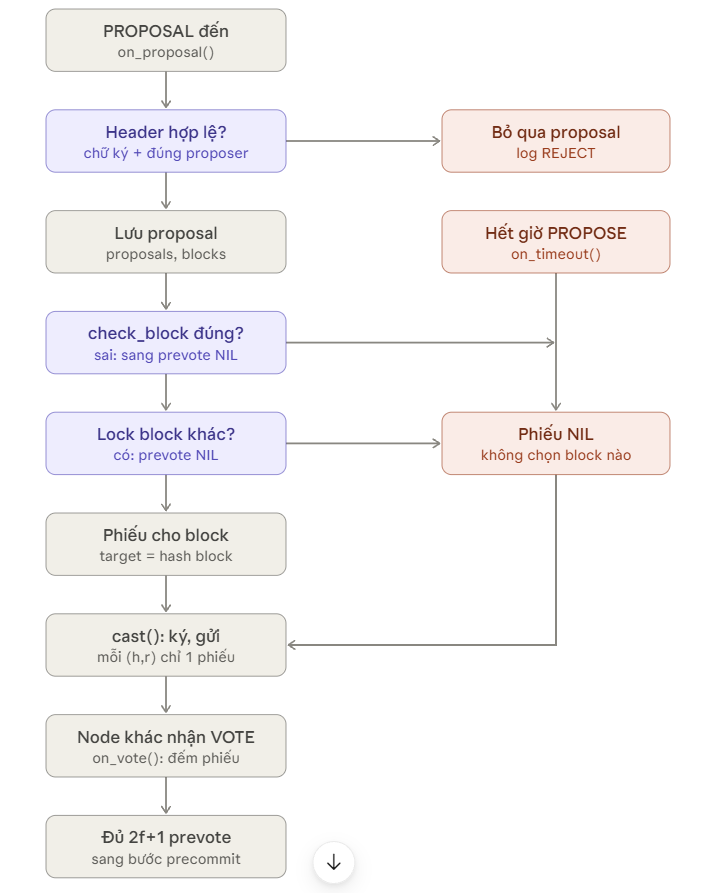
\includegraphics[width=0.45\textwidth,height=0.45\textheight,keepaspectratio]{prism-uploads/image_3.png}
    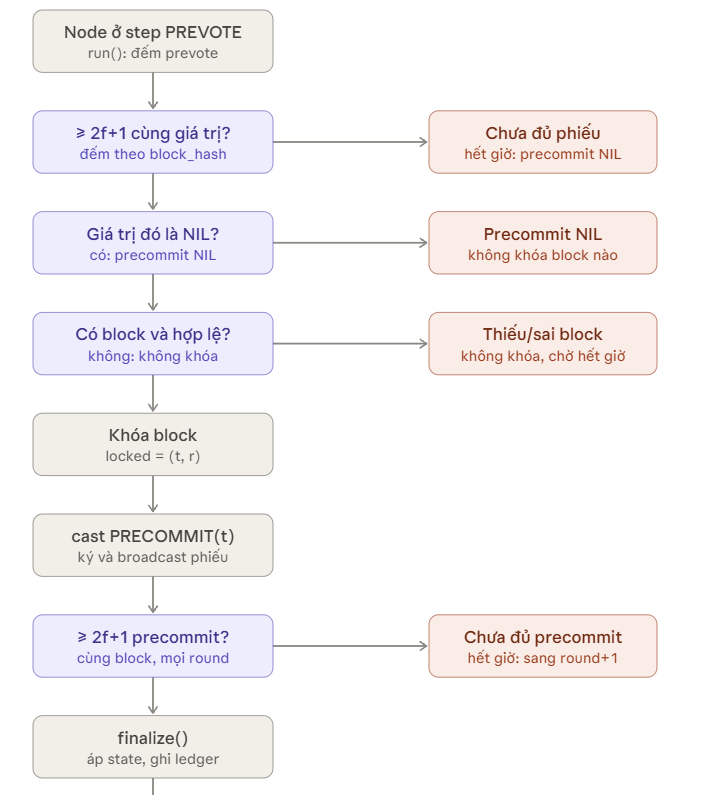
\includegraphics[width=0.45\textwidth,height=0.45\textheight,keepaspectratio]{prism-uploads/image.png}

\subsection{Đồng bộ catch-up}
\begin{figure}[H]
    \centering
    \begin{tikzpicture}[scale=0.8,x=1cm,y=0.85cm,transform shape,>=stealth,every node/.style={font=\small}]
        \tikzstyle{syncstep}=[draw,rounded corners,align=center,text width=7.2cm,minimum height=0.72cm,inner sep=3pt]
        \node[syncstep,fill=gray!10] (start) at (0,0) {Validator B bị chậm\\Height hiện tại = 7};
        \node[syncstep,fill=blue!6] (detect) at (0,-1.3) {Phát hiện validator A đã commit đến height 10};
        \node[syncstep,fill=gray!10] (request) at (0,-2.6) {Gửi \texttt{SYNC\_REQ}\\Yêu cầu height 8 đến 10};
        \node[syncstep,fill=gray!10] (receive) at (0,-3.9) {Validator A nhận yêu cầu};
        \node[syncstep,fill=gray!10] (headers) at (0,-5.2) {A gửi \texttt{SYNC\_HEADERS}\\Header kèm CommitCertificate};
        \node[syncstep,fill=blue!6] (verify) at (0,-6.5) {B xác minh header, chữ ký và certificate};
        \node[syncstep,fill=gray!10] (bodyrequest) at (0,-7.8) {B yêu cầu \texttt{REQUEST\_BODY}};
        \node[syncstep,fill=gray!10] (body) at (0,-9.1) {Nhận BODY / \texttt{SYNC\_RESP}};
        \node[syncstep,fill=blue!6] (check) at (0,-10.4) {Kiểm tra \texttt{tx\_root}, thực thi giao dịch\\và kiểm tra \texttt{state\_hash}};
        \node[syncstep,fill=blue!10] (decision) at (0,-11.7) {Dữ liệu hợp lệ?};
        \node[syncstep,fill=green!10] (ledger) at (-4.2,-13.2) {Có: cập nhật ledger};
        \node[syncstep,fill=red!10] (reject) at (4.2,-13.2) {Không: từ chối dữ liệu không hợp lệ};
        \node[syncstep,fill=gray!10] (continue) at (-4.2,-14.5) {Tiếp tục đồng bộ block còn thiếu};
        \node[syncstep,fill=green!10] (caughtup) at (-4.2,-15.8) {Bắt kịp blockchain};
        \draw[->] (start.south) -- (detect.north);
        \draw[->] (detect.south) -- (request.north);
        \draw[->] (request.south) -- (receive.north);
        \draw[->] (receive.south) -- (headers.north);
        \draw[->] (headers.south) -- (verify.north);
        \draw[->] (verify.south) -- (bodyrequest.north);
        \draw[->] (bodyrequest.south) -- (body.north);
        \draw[->] (body.south) -- (check.north);
        \draw[->] (check.south) -- (decision.north);
        \draw[->] (decision.south west) -- node[pos=0.5,above left]{Có} (ledger.north);
        \draw[->] (decision.south east) -- node[pos=0.5,above right]{Không} (reject.north);
        \draw[->] (ledger.south) -- (continue.north);
        \draw[->] (continue.south) -- (caughtup.north);
    \end{tikzpicture}
    \caption{Quy trình catch-up bằng header, certificate và body}
    \label{fig:catchup-headers-body}
\end{figure}
\subsection{Mô hình mạng mô phỏng}
Tầng mạng được triển khai trong \texttt{src/sim.py} thông qua lớp \texttt{Net}, theo mô hình mô phỏng sự kiện rời rạc (Discrete-Event Simulation). Các node trao đổi thông điệp bằng các hàm \texttt{send()} và \texttt{broadcast()}. Hàng đợi ưu tiên cùng đồng hồ ảo giúp mô phỏng có tính tất định.

\paragraph{Mô phỏng lỗi mạng.} Mạng hỗ trợ các lỗi trễ (Delay), mất gói (Drop), nhân bản (Duplicate) và đảo thứ tự (Reorder) theo xác suất cấu hình. Trước GST, mạng có thể không ổn định; sau GST, độ trễ truyền dẫn được giới hạn bởi $\Delta$, không tính thời gian chờ do giới hạn tốc độ gửi (Rate Limiting) hoặc chặn peer (Peer Blocking).

\paragraph{Giới hạn tốc độ gửi và chặn peer.} Hệ thống giới hạn số thông điệp gửi trên mỗi kết nối, trì hoãn các thông điệp vượt ngưỡng và hỗ trợ chặn hoặc bỏ chặn peer theo thời gian cấu hình.

\paragraph{Topology.} Hệ thống hỗ trợ cấu trúc full mesh hoặc danh sách liên kết tùy chỉnh, với độ trễ riêng cho từng liên kết thông qua \texttt{link\_delays}.

\paragraph{Ghi nhật ký mạng.} Hệ thống ghi nhận các sự kiện \texttt{SEND}, \texttt{DROP}, \texttt{DELAY}, \texttt{DUPLICATE}, \texttt{BLOCK} và \texttt{UNBLOCK}.
\subsection{Mô hình Byzantine}
\label{sec:byzantine-model}

Mỗi hành vi Byzantine là một lớp con của \texttt{Node} trong \texttt{src/byzantine.py}. Lớp con chỉ ghi đè đúng hàm cần làm sai; phần còn lại vẫn chạy như node trung thực. Ba nguyên tắc: (1) chỉ ký bằng khóa của chính nó, không giả chữ ký người khác; (2) chỉ tác động lên node khác qua mạng, không sửa trực tiếp dữ liệu của node khác; (3) cấu hình tấn công xong trước khi node bắt đầu chạy.

\begin{table}[H]
\centering
\small
\begin{tabularx}{\textwidth}{|p{3.5cm}|X|p{3.6cm}|}
\hline
\textbf{Lớp} & \textbf{Làm sai thế nào} & \textbf{Node trung thực chặn bằng} \\
\hline
\texttt{Silent} & Không gửi gì (chết hẳn), hoặc vẫn bỏ phiếu nhưng không đề xuất block. & Timeout rồi sang round mới. \\
\hline
\texttt{EquivocateVoter} & Ký hai phiếu khác nhau cho cùng (height, round, loại phiếu). & Chỉ đếm phiếu đến trước, log \texttt{EQUIVOCATION}. \\
\hline
\texttt{EquivocateProposer} & Đề xuất hai block hợp lệ khác nhau cho cùng (height, round). & Prevote block đến trước, log \texttt{EQUIVOCATION}. \\
\hline
\texttt{InvalidBlock} & Header ký đúng nhưng nội dung sai đúng một chỗ (parent, \texttt{tx\_root}, \texttt{state\_hash}, chữ ký tx, tx lặp, \texttt{pol\_round}). & Kiểm tra block, log \texttt{REJECT} đúng lý do, prevote NIL. \\
\hline
\texttt{Replay} & Gửi lại nguyên vẹn tin cũ (cùng chữ ký) sau một khoảng trễ. & Mỗi người chỉ một phiếu mỗi slot; tin quá cũ bị bỏ. \\
\hline
\texttt{ForkCoalition} & Cả nhóm Byzantine cùng ký cho hai block, gửi mỗi block cho một nửa mạng. & Chỉ dùng cho thí nghiệm $n=9$ ngoài giả định. \\
\hline
\end{tabularx}
\caption{Các hành vi Byzantine được mô phỏng}
\label{tab:byzantine}
\end{table}

Bật hành vi Byzantine bằng mục \texttt{"byzantine"} trong file cấu hình, ví dụ \texttt{\{"1": \{"behavior": "silent"\}\}}. Test nào dùng hành vi nào được nêu ở Mục~\ref{sec:testing}.
